\documentclass[10pt]{article}
\usepackage[margin=10pt]{geometry}
\usepackage[utf8]{inputenc}
\usepackage[english, greek]{babel}
\usepackage{comment}
\usepackage{amsmath}
\usepackage{amssymb}
\usepackage{graphicx}
\graphicspath{ {./imgs/} }
\usepackage{listing}
\usepackage{float}

\newcommand{\lat}{\foreignlanguage{english}}
\newcommand{\ABox}{\foreignlanguage{english}{ABox}}
\newcommand{\TBox}{\foreignlanguage{english}{TBox}}
\newcommand{\RBox}{\foreignlanguage{english}{RBox}}

\newcommand{\yp}{\sqsubseteq}
\newcommand{\kai}{\sqcap}
\newcommand{\h}{\sqcup}
%%%%%%%%%%%%%%%%%%%%%%%%%%%%%%%%%%%%%%%%%%%%%%%%%%%%%%%%%%%%%%%%%%%%%%%%%%%%%%%%%
\title{Συστήματα και Τεχνολογίες Γνώσης\\ \small{2η Γραπτή Εργασία}}
\author{Όνομα: Ευστράτιος Καραπαναγιώτης\\ \small{ΑΜ: 03115177}}

\begin{document}
	\maketitle
	
	\section*{Ερώτημα 1}
	Αρχικά μετατρέπουμε τις έννοιες $C_1, C_2$ της περιγραφικής λογικής $FL_0$ σε κανονική μορφή. Έχουμε διαδοχικά:
	\begin{itemize}
		\item $C_1 \equiv D \sqcap E \sqcap \forall r.(A \sqcap \forall r.E \sqcap B \sqcap (A \sqcap B) \sqcap \forall r.\forall s.D) \equiv D \sqcap E \sqcap \forall r.(A \sqcap B \sqcap \forall r. (E \sqcap \forall s.D))$
		
		\item $C_2 \equiv E \sqcap \forall r.(\forall r.(E \sqcap B) \sqcap \forall r.\forall s.(D \sqcap A)) \equiv E \sqcap \forall r.(\forall r.(E \sqcap B \sqcap \forall s.(D \sqcap A)) \equiv E \sqcap \forall r.(\forall r.(E \sqcap B \sqcap \forall s.D \sqcap \forall s.A))$
	\end{itemize}

	Στη συνέχεια εφαρμόζουμε τον αλγόριθμο δομικής υπαγωγής για τη γλώσσα $FL_0$.
	
	\begin{enumerate}
		\item \textbf{\lat{Extract($C_1$, $C_2$)}} 
		$\begin{cases}
		NC = \{D, E\} \\
		ND = \{E\} \\
		RC = \{r\} \\
		RD = \{r\} \\
		\end{cases}$
		
		\item \textbf{\lat{$1^{st}$ Condition}} Διατρέχουμε τα στοιχεία του \lat{ND} και ελέγχουμε αν ανήκουν και στο σύνολο \lat{NC}. Το μοναδικό στοιχείο το οποίο υπάρχει είναι το Ε, το οποίο είναι μέλος και στο σύνολο \lat{NC}. Επομένως, ικανοποιείται η πρώτη συνθήκη.
		
		\item \textbf{\lat{$2^{nd}$ Condition}} Στο σημείο αυτό για κάθε στοιχείο-ρόλο στο σύνολο \lat{RD} απογυμνώνουμε τη σύνθετη έννοια με την οποία είναι συνδεδεμένη ο ρόλος και για τις δύο αρχικές έννοιες. Για παράδειγμα: $\forall r \in ND; \ do \ X := strip(C_1, r); Y := strip(C_2, r); \ done$. Οι έννοιες \lat{X, Y} είναι οι σύνθετες έννοιες που ήταν συνδεδεμένες με τον ρόλο \lat{r} για να κατασκευάσουν μια έννοια. Στην περίπτωσή μας, $X \equiv A \sqcap B \sqcap \forall r. (E \sqcap \forall s.D)$ και $Y \equiv \forall r.(E \sqcap B \sqcap \forall s.D \sqcap \forall s.A)$. Στη συνέχεια εκτελούμε για τις έννοιες \lat{X, Y} έλεγχο με τον ίδιο αλγόριθμο για την υπαγωή της \lat{X} στην \lat{Y}.
		
		\item \textbf{\lat{Extract($X$, $Y$)}}
		$\begin{cases}
		NC = \{A, B\} \\
		ND = \{\} \\
		RC = \{r\} \\
		RD = \{r\} \\
		\end{cases}$

		\item \textbf{\lat{$1^{st}$ Condition}} Δεν υπάρχει κάποιο στοιχείο στο σύνολο \lat{ND} να διατρέξουμε οπότε η πρώτη συνθήκη ικανοποιείται.
		
		\item \textbf{\lat{$2^{nd}$ Condition}}	Παίρνουμε $X' \equiv E \sqcap \forall s.D$ και $Y' \equiv E \sqcap B \sqcap \forall s.D \sqcap \forall s.A$. Εφαρμόζουμε, ξανά, αναδρομικά τον αλγόριθμο απόδειξης της δομικής υπαγωγής στα $X'$ και $Y'$.
		
		\item \textbf{\lat{Extract($X'$, $Y'$)}}
		$\begin{cases}
		NC = \{E\} \\
		ND = \{E, B\} \\
		RC = \{s\} \\
		RD = \{s\} \\
		\end{cases}$

		\item \textbf{\lat{$1^{st}$ Condition}} Αυτη τη φορά βλέπουμε ότι δεν ικανοποιείται η συνθήκη επειδή παρόλο που το Ε ανήκει και στο σύνολο \lat{NC}, το Β \textbf{δεν} ανήκει. Έτσι, δεν ισχύει $X' \sqsubseteq Y'$.
		
		\item \textbf{Επιστροφή} Επιστρέφεται στην προηγούμενη κλήση το αποτέλεσμα $NO$ το οποίο με τη σειρά του πυροδοτεί την επιστροφή ενός $NO$ στην πρώτη αναδρομική κλήση. 
		
	\end{enumerate}

	Επομένως, καταλήγουμε με βάση τον αλγόριθμο δομικής υπαγωγής πως \textbf{δεν} ισχύει η υπαγωγή $C_1 \sqsubseteq C_2$.
	
	\section*{Ερώτημα 2}
	\begin{enumerate}
		\item \textbf{ΚΜΑ και απαλοιφή \TBox} \\
		Παρατηρούμε ότι για η σχέση στο \TBox \ δεν είναι απλή όπως και η πρόταση που προσπαθούμε να αποδείξουμε ότι ισχύει. Για το λόγο αυτό χρησιμοποιούμε και για τις δύο προτάσεις την απαλοιφή με χρήση της τεχνικής της εσωτερίκευσης.\\\\
		$\neg A \yp \exists R.B \rightarrow (A \h \exists R.B)(a)$\\
		$\forall R. \neg B \yp A \rightarrow (\exists R.B \h A)(a)$\\\\
		Έχουμε λοιπόν ως αρχικό ταμπλό το $S_0 = \{\{(A \h \exists R.B)(a), (\exists R.B \h A)(a)\}\}$. Βλέπουμε ότι αφορούν την ίδια έννοια και επομένως αφού τα \lat{ABoxes} είναι σύνολα ισχυρισμών λόγω του ορισμού των συνόλων τα επαναλαμβανόμενα στοιχεία παραλείπονται. Έτσι, $S_0 =  \{\{(A \h \exists R.B)(a)\} \}$. 
		%Προσπέλαση των στοιχείων του ταμπλό Θα γίνεται με την γραφή $S_i[j] , \ \forall A_j \in S_i$. 
		
		\textbf{Επέκταση Ταμπλό}
		\begin{enumerate}
			\item Κανόνας $K_{\h}$:\\\\ $S_1 = \{ \{(A \h \exists R.B)(a) , A(a)\} , \{(A \h \exists R.B)(a), (\exists R.B)(a)\} \}$\\
			
			\item Κανόνας $K_{\exists}$ και εσωτερίκευση:\\\\ $S_2 = \{ \{(A \h \exists R.B)(a) , A(a)\} , \{(A \h \exists R.B)(a), (\exists R.B)(a), R(a, x_1), B(x_1), (A \h \exists R.B)(x_1) \} \}$\\
			
			\item Κανόνας $K_{\h}$:\\\\ 
			$S_3 = \{ \{(A \h \exists R.B)(a) , A(a)\} ,\{(A \h \exists R.B)(a), (\exists R.B)(a), R(a, x_1), B(x_1), (A \h \exists R.B)(x_1) , A(x_1) \} ,\\ \{(A \h \exists R.B)(a), (\exists R.B)(a), R(a, x_1), B(x_1), (A \h \exists R.B)(x_1) , (\exists R.B)(x_1) \} \}$\\
			
			\item Κανόνας $K_{\exists}$ και εσωτερίκευση:\\\\ $S_4 = \{ \{(A \h \exists R.B)(a) , A(a)\} ,\\ \{(A \h \exists R.B)(a), (\exists R.B)(a), R(a, x_1), B(x_1), (A \h \exists R.B)(x_1) , A(x_1) \} ,\\ \{(A \h \exists R.B)(a), (\exists R.B)(a), R(a, x_1), B(x_1), (A \h \exists R.B)(x_1) , (\exists R.B)(x_1), R(x_1, x_2), B(x_2), (A \h \exists R.B)(x_2) \} \}$\\
			
			\item \lat{Blocking}: ο αλγόριθμος παρατηρεί ότι το πλήθος των νέων παιδών με την εφαρμογή του προηγούμενου βήματος είναι τρία. Το ίδιο ισχύει και όταν εφαρμόστηκε ο κανόνας $K_{\exists}$ σε συνδιασμό με την ιδιότητα της εσωτερίκευσης για το $x_1$. Επομένως, σταματάει η επέκταση του ταμπλό και θεωρείται πλήρες.

		\end{enumerate}
		
		\textbf{Εύρεση \ABox \ το οποίο δεν περιέχει αντιφάσεις}\\
		Κατευθείαν βλέπουμε ότι το πρώτο \ABox \ του ταμπλό $S_4$ δεν παρουσιάζει αντιφάσεις. Επομένως, ισχύει η πρόταση $\neg A \yp \exists R.B$ για το \TBox \ $\forall R. \neg B \yp A$.
		
		\item \textbf{ΚΜΑ και απαλοιφή \TBox} \\
		Παρατηρούμε ότι το \TBox \ δεν είναι ακυκλικό καθώς $u(A, C) = 1$ και $u(C, A) = 1$. Οπότε $u'(A, A) = 2 \neq 0$. Για το λόγο αυτό θα χρησιμοποιηθεί ξανά η διαδικασία της εσωτερίκευσης για την απαλοιφή του \TBox.
		$
		\begin{cases}
		1.\ A \yp C \Rightarrow (\neg A \h C)(x) \\
		2.\ C \yp \exists R.D \Rightarrow (\neg C \h \exists R.D)(x) \\
		3.\ D \yp \neg A \Rightarrow (\neg D \h \neg A)(x) \\
		4.\ C \yp \forall R.A \Rightarrow (\neg C \h \forall R.A)(x)
		\end{cases}
		$
		
		Έτσι, το ταμπλό αρχικοποιείται στο στιγμιότυπο: $S_0 = \{\{A(a), R(a, b), (\neg A \h C)(a), (\neg A \h C)(b), (\neg C \h \exists R.D)(a),\\ (\neg C \h \exists R.D)(b), (\neg D \h \neg A)(a), (\neg D \h \neg A)(b), (\neg C \h \forall R.A)(a), (\neg C \h \forall R.A)(b)\} \}$\\
		
		Ονομάζουμε το πρώτο \ABox \ ως $A_0$ για να γίνει πιο κατανοητή και εκφρασιτκή η διαδικασία.
		
		\textbf{Επέκταση Ταμπλό}
		\begin{enumerate}
			\item Κανόνας $K_{\h}$ για την έννοια (1) και για τα δύο άτομα $a, b$: \\\\ 
			$S_1 = \{ A_0\cup\{\neg A(a), \neg A(b)\} , A_0\cup\{\neg A(a), C(b)\} , A_0\cup\{C(a), \neg A(b)\} , A_0\cup\{C(a), C(b)\} \}$.\\\\
			Πλέον φαίνεται ότι ικανοποιούνται οι συνθήκες για την έννοια (3) οπότε δεν μπορεί να επεκτείνει κάτι. Επίσης αποφεύγουμε την επέκταση του ταμπλό μέσω της 2 καθώς θα προσθέσει επιπλέον άτομο και οπότε λόγω της ιδιότητας της εσωτερίκευσης θα έχουμε μεγαλύτερα ταμπλό και όχι κάποια σημαντική νέα πληροφορία.\\
			
			\item Κανόνας $K_{\h}$ για την έννοια (4) και για το άτομο $a$:\\\\ $S_2 = \{  A_0\cup\{\neg A(a), \neg A(b), \neg C(a)\}, A_0\cup\{\neg A(a), \neg A(b), (\forall R.A)(a)\} , A_0\cup\{\neg A(a), C(b), C(a)\}, A_0\cup\{\neg A(a), C(b), \\ (\forall R.A)(a)\} , A_0\cup\{C(a), \neg A(b), \neg C(a)\}, A_0\cup\{C(a), \neg A(b), (\forall R.A)(a)\} , A_0\cup\{C(a), C(b), \neg C(a)\}, A_0\cup\{C(a), C(b), (\forall R.A)(a)\} \}$\\
			
			\item Κανόνας $K_{\forall}$:\\\\ $S_3 = \{  A_0\cup\{\neg A(a), \neg A(b), \neg C(a)\}, A_0\cup\{\neg A(a), \neg A(b), (\forall R.A)(a), A(b)\} , A_0\cup\{\neg A(a), C(b), C(a)\},\\ A_0\cup\{\neg A(a), C(b), (\forall R.A)(a), A(b)\} , A_0\cup\{C(a), \neg A(b), \neg C(a)\}, A_0\cup\{C(a), \neg A(b), (\forall R.A)(a), A(b)\} ,\\ A_0\cup\{C(a), C(b), \neg C(a)\}, A_0\cup\{C(a), C(b), (\forall R.A)(a), A(b)\} \}$\\
			
			\item Κανόνας $K_{\h}$ για την έννοια (4) και για το άτομο $b$:\\\\
			$ S_4 = \{
			\begin{cases}
			1.\ A_0\cup\{\neg A(a), \neg A(b), \neg C(a), \neg C(b)\},\\
			2.\ A_0\cup\{\neg A(a), \neg A(b), \neg C(a), (\forall R.A)(b)\},\\
			
			3.\ A_0\cup\{\neg A(a), \neg A(b), (\forall R.A)(a), A(b), \neg C(b)\},\\
			4.\ A_0\cup\{\neg A(a), \neg A(b), (\forall R.A)(a), A(b), (\forall R.A)(b)\},\\
			
			5.\ A_0\cup\{\neg A(a), C(b), C(a), \neg C(b)\},\\
			6.\ A_0\cup\{\neg A(a), C(b), C(a), (\forall R.A)(b)\},\\
			
			7.\ A_0\cup\{\neg A(a), C(b), (\forall R.A)(a), A(b), \neg C(b)\},\\
			8.\ A_0\cup\{\neg A(a), C(b), (\forall R.A)(a), A(b), (\forall R.A)(b)\},\\
			
			9.\ A_0\cup\{C(a), \neg A(b), \neg C(a), \neg C(b)\},\\
			10.\ A_0\cup\{C(a), \neg A(b), \neg C(a), (\forall R.A)(b)\},\\
			
			11.\ A_0\cup\{C(a), \neg A(b), (\forall R.A)(a), A(b), \neg C(b)\},\\
			12.\ A_0\cup\{C(a), \neg A(b), (\forall R.A)(a), A(b), (\forall R.A)(b)\},\\
			
			13.\ A_0\cup\{C(a), C(b), \neg C(a), \neg C(b)\},\\
			14.\ A_0\cup\{C(a), C(b), \neg C(a), (\forall R.A)(b)\},\\
			
			15.\ A_0\cup\{C(a), C(b), (\forall R.A)(a), A(b), \neg C(b)\},\\
			16.\ A_0\cup\{C(a), C(b), (\forall R.A)(a), A(b), (\forall R.A)(b)\}						
			\end{cases}
			\}
			$\\
			
			\item Δεν υπάρχει άλλη επέκταση (κάποιος κανόνας που μπορεί να εφαρμοστεί) για το ταμπλό, οπότε η παραπάνω μορφή είναι η τελική.
		\end{enumerate}
		
		\textbf{Εύρεση \ABox \ το οποίο δεν περιέχει αντιφάσεις}\\
		Όλα τα \ABox ,\ από το 1 εώς το 15 περιέχουν αντιφάσεις. Το μοναδικό το οποίο δεν περιέχει αντιφάσεις είναι το 16ο \ABox. Επομένως, το \ABox \ $A = \{A(a), R(a, b)\}$ είναι ικανοποιήσιμο για το \TBox \ που δίνεται.
	\end{enumerate}
	
	\section*{Ερώτημα 3}
	\begin{enumerate}
		\item Σε πρώτη φάση παρουσιάζεται ο συνολικός \lat{RDFS} γράφος στην εικόνα \ref{rdfsgraph}. Με βάση αυτόν θα δοθεί η απάντηση για τον \lat{RDFS reasoner}.
		
		\begin{figure}[H]
		\centering
		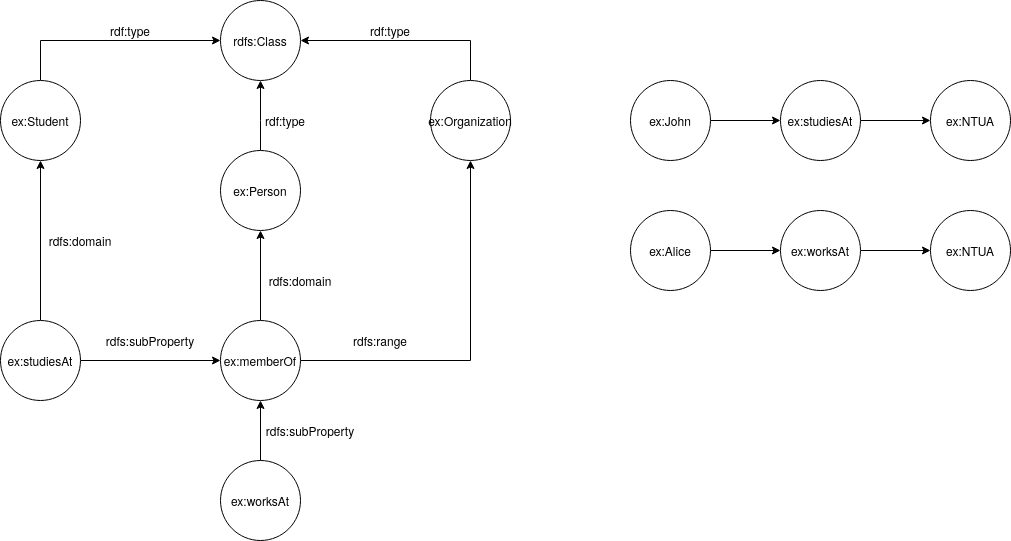
\includegraphics[scale=0.4]{question3}
		\caption{\footnotesize{Ο \lat{RDFS} γράφος της βάσης γνώσης}}
		\label{rdfsgraph}
		\end{figure}

		Για την πρώτη πρόταση γνωρίζει ότι το \lat{ex:studiesAt} είναι υπορόλος της \lat{ex:memberOf} μέσω της σχέσης \lat{ex:subProperty}. Η \lat{ex:subProperty} δέχεται ως ορίσματα όμως δύο σχέσεις(ρόλους). Η \lat{ex:studiesAt} όμως είναι το ένα όρισμά της και έτσι συνάγει ότι:\\ \textbf{\lat{ex:studiesAt a rdfs:Property}}.
		
		Για τη δεύτερη πρόταση γνωρίζει ότι ο \lat{ex:John} σπουδάζει(\lat{ex:studiesAt}) στο ΕΜΠ (\lat{ex:NTUA}). Για το ρόλο \lat{ex:studiesAt} γνωρίζει ότι έχει ως πεδίο ορισμού το \lat{ex:Student}. Επομένως, το \lat{ex:John} είναι μέλος της έννοιας \lat{ex:Student}. Η έννοια \lat{ex:Student} είναι όμως υποέννοια της \lat{ex:Person}. Προκύπτει λοιπόν ότι το \lat{ex:John} είναι μέλος (υπάγεται) της έννοιας \lat{ex:Person} και συνάγει ότι:\\ \textbf{\lat{ex:John a ex:Person}}.
	
		\item Το ερώτημα \lat{SPARQL} διατυπώνεται ως εξής:
		
		\begin{listing}
			\lat{\textbf{SELECT} ?organization ?name}\\
			\lat{\textbf{WHERE}}\\
			\{\\
				\lat{?organization rdf:type ex:Organization}\\
				\lat{?name ex:memberOf ?organization}\\
			\}
		\end{listing}
	
		Θα πρέπει να σημειωθεί ότι το παραπάνω \lat{SPARQL} ερώτημα επιστρέφει οποιοδήποτε όνομα αντικειμένου είναι μέλος του οργανισμού \lat{?organization}. Επιτρέπει δηλαδή εκτός από ανθρώπους και άλλα άτομα. Για παράδειγμα ακόμα και μια εταιρεία μπορεί να συμμετέχει σε έναν οργανισμό. Επίσης, δεν διακρίνει αυτούς που εργάζονται από τους υπόλοιπους. Έτσι, κάποιος μπορεί να είναι μέλος (π.χ. μέτοχος) αλλά να μην εργάζεται για τον οργανισμό αυτόν.
	\end{enumerate}
	
	\section*{Ερώτημα 4}
	\begin{enumerate}
		\item 
		\begin{itemize}
			\item \lat{ex:Place owl:disjointWith ex:Person}. $\rightarrow$ \lat{DisjointClasses(ex:Place, ex:Person)}.
			
			\item \lat{ex:livesIn rdfs:domain ex:Person} $\rightarrow$ \lat{ObjectPropertyDomain(ex:livesin, ex:Person)}
			
			\item \lat{ex:livesIn rdfs:range ex:Place} $\rightarrow$ \lat{ObjectPropertyRange(ex:livesIn, ex:Place)}
			
			\item \lat{ex:John ex:livesIn ex:Athens} $\rightarrow$ \lat{ObjectPropertyAssertion(ex:livesIn, ex:John, ex:Athens)}
			
			\item \lat{ex:Athens a \_:b1} $\rightarrow$ \lat{ClassAssertion(\_:b1, ex:John)}
			
			\item \lat{\_:b1 owl:complementOf ex:Person} $\rightarrow$ \lat{equivalentClasses(\_:b1, complementOf(ex:Person))}	
		\end{itemize}
	
		\item \textbf{ΚΜΑ και απαλοιφή \TBox} \\
		Αρχικά γίνεται απεικόνιση της βάσης γνώσης στα αντίστοιχα σώματα \ABox \ και \TBox. Επομένως, $ABox = \{livesIn(John, Athens)\}$ και $TBox = \{\exists livesIn \yp Person, \exists livesIn^{-} \yp Place, Person \kai Place \yp \bot \}$. Οι δύο τελευταίες τριάδες εκφράζονται ως $b_1(Athens)$ και $b_1 \equiv \neg Person$. Κατά τα γνωστά, θα πρέπει να ενσωματωθεί το \TBox \ στο \ABox \ προκειμένου να μπορεί να ξεκινήσει η εκτέλεση του αλγορίθμου \lat{tableau}. Επειδή, οι δηλώσεις στο \TBox \ δεν είναι απλής μορφής χρησιμοποείται η μέθοδος της εσωτερίκευσης.\\\\
		Δηλαδή
		$
		\begin{cases}
		1.\ \exists livesIn \yp Person \Rightarrow ((\forall livesIn.\bot ) \h Person)(a)\\
		
		2.\ \exists livesIn^{-} \yp Place \Rightarrow ((\forall livesIn^{-}.\bot ) \h Place)(a)\\
		
		3.\ Person \kai Place \yp \bot \Rightarrow (\neg Person \h \neg Place)(a)
		\end{cases}
		$\\\\
		Προκύπτει λοιπόν το πρώτο στιγμιότυπο του ταμπλό $S_0 = \{ \{livesIn(John, Athens), ((\forall livesIn.\bot ) \h Person)(a), ((\forall livesIn^{-}.\bot ) \h Place)(a), (\neg Person \h \neg Place)(a), \neg Person(Athens) \} \}$, όπου χρησιμοποιήθηκε απευθείας η μέθοδος ξεδιπλώματος για τα $b_1(Athens)$ και $b_1 \equiv \neg Perosn$.
		
		\textbf{Επέκταση Ταμπλό}\\
		Χρησιμοποιείται ο συμβολισμός $A_0$ για να δηλωθεί το αρχικό \ABox \ που κατασκευάστηκε για τον αλγόριθμο.
		\begin{enumerate}
			\item Κανόνας $K_{\h}$ για την (1):\\\\ 
			$S_1 = \{ A_0\cup\{(\forall livesIn.\bot)(a)\} , A_0\cup\{Person(a)\} \}$\\
			
			\item Κανόνας $K_{\h}$ για την (2):\\\\ 
			$S_2 = \{ A_0\cup\{ (\forall livesIn.\bot)(a), (\forall livesIn^{-}.\bot)(a) \} ,
			A_0\cup\{ (\forall livesIn.\bot)(a), Place(a) \} ,
			A_0\cup\{Person(a), (\forall livesIn.\bot)(a)\} , 
			A_0\cup\{Person(a), Place(a)\} \}$\\
			
			\item Κανόνας $K_{\h}$ για την (3):\\\\ 
			$S_2 = \{
			\begin{cases}
			
			1.\ A_0\cup\{ (\forall livesIn.\bot)(a), (\forall livesIn^{-}.\bot)(a), \neg Person(a)\},\\
			2.\ A_0\cup\{ (\forall livesIn.\bot)(a), (\forall livesIn^{-}.\bot)(a), \neg Place(a)\},\\
			
			3.\ A_0\cup\{ (\forall livesIn.\bot)(a), Place(a), \neg Person(a) \},\\
			4.\ A_0\cup\{ (\forall livesIn.\bot)(a), Place(a), \neg Place(a) \},\\
			
			5.\ A_0\cup\{Person(a), (\forall livesIn.\bot)(a), \neg Person(a)\},\\
			6.\ A_0\cup\{Person(a), (\forall livesIn.\bot)(a), \neg Place(a)\},\\
			
			7.\ A_0\cup\{Person(a), Place(a), \neg Person(a)\}\\
			8.\ A_0\cup\{Person(a), Place(a), \neg Place(a)\}\\
			
			\end{cases}
			\}$\\
			
			\item Δεν υπάρχει άλλη επέκταση (κάποιος κανόνας που μπορεί να εφαρμοστεί) για το ταμπλό, οπότε η παραπάνω μορφή είναι η τελική.
		\end{enumerate}
	
		\textbf{Εύρεση \ABox \ το οποίο δεν περιέχει αντιφάσεις}\\
		Το πρώτο κι ολας \ABox \ δεν παρουσιάζει αντιφάσεις και έτσι ο \lat{OWL reasoner} αποδεικνύει ότι οι δύο τελυταίες προτάσεις είναι συμπέρασμα των προηγούμενων. 
	\end{enumerate}
\end{document}